\documentclass[main]{subfiles}
\begin{document}

%@@@@@@@@@@@@@@@@@@@@@@@@@@@@@@
% Main Topics: barrier functions and central path
% Interior Point Methods - 30.10.2017
% author: Vanessa Leite

\section{Interior Point Methods}

\subsection{Preliminaries}

\paragraph{Lemma: Let $f$ ba a function. $dom(f) \mapsto \mathbb{R}$ convex
and continuously differentiable. Then, for $x^* \in dom(f)$:
$f(x^*) = \displaystyle \min_{x \in dom(f)} f(x) \iff \nabla f(x^*) = 0$}

\paragraph{Observation: In $\mathbb{Z}$ we do not have a criteria like this.}
Proof on lecture 13.

\paragraph{Lemma: Assume $f$ strictly convex. Suppose $Q$ is the domain,
$Q \subseteq dom(f)$ is compact, (i.e, if you take a sequence, look to the
limit, limit lies on the sequence). $Q$ is convex. Then, there exists a unique
$x^* \in Q$ such that $f(x^*) = \displaystyle \min_{x \in Q} f(x)$.}

\subparagraph{Proof:}
The existence of $x^*$ follows from compacteness of $Q \subseteq dom (f)$. For
$x, y \in Q$, $x \neq y$, let $x = \frac{1}{2}x + \frac{1}{2}y$. Then, from the
strictly convexity, $f(z) < \frac{1}{2} f(x) + \frac{1}{2} f(y) \leq max \{f(x),
f(y) \}$. This implies that both $x$ and $y$ cannot be minimizers.

\subsection{Logarithmic Barriers}
Consider primal-dual pair of linear optimization problems:
Primal (P) $p^* = \max \{c^T x \mid Ax = b, x \geq 0 \}$.
Dual (D) $d^* = \min \{b^T y x \mid A^T y, y \in \mathbb{R}^m \}$.

Assumptions:
\begin{itemize}
\item $A$ has full row rank (i.e., looking  at the rows of the linear system,
either we can remove redundant constraints or the problem is (in?)feasible).
\item $D = \{ y \in \mathbb{R}^m \mid A^T y \geq c \}$ is bounded (test
recession cone $A^T y \geq 0$, farka's lemma).
\item There exists an "interior point" in $D$, i.e., $\exists y$ such that
$\underbrace{A^T y > c}_{\text{component-wise}}$. I.e., the polyhedron is "full
dimensional".
\end{itemize}

\paragraph{Definition: Consider the function $\phi: \mathbb{R}^m \mapsto
\mathbb{R}$. $\phi(y) = - \sum_{j=1}^{n} log (y^T A_{\cdot j} - c_j)$ is
called a \emph{log barrier for $D$}.}
Log barrier only works for the dual. \\

The log barrier method prevents to reach the boundary, so, it prevents to reach
a vertex. \\

\begin{figure}[!h]
  \label{fig:projection}
  \centering
    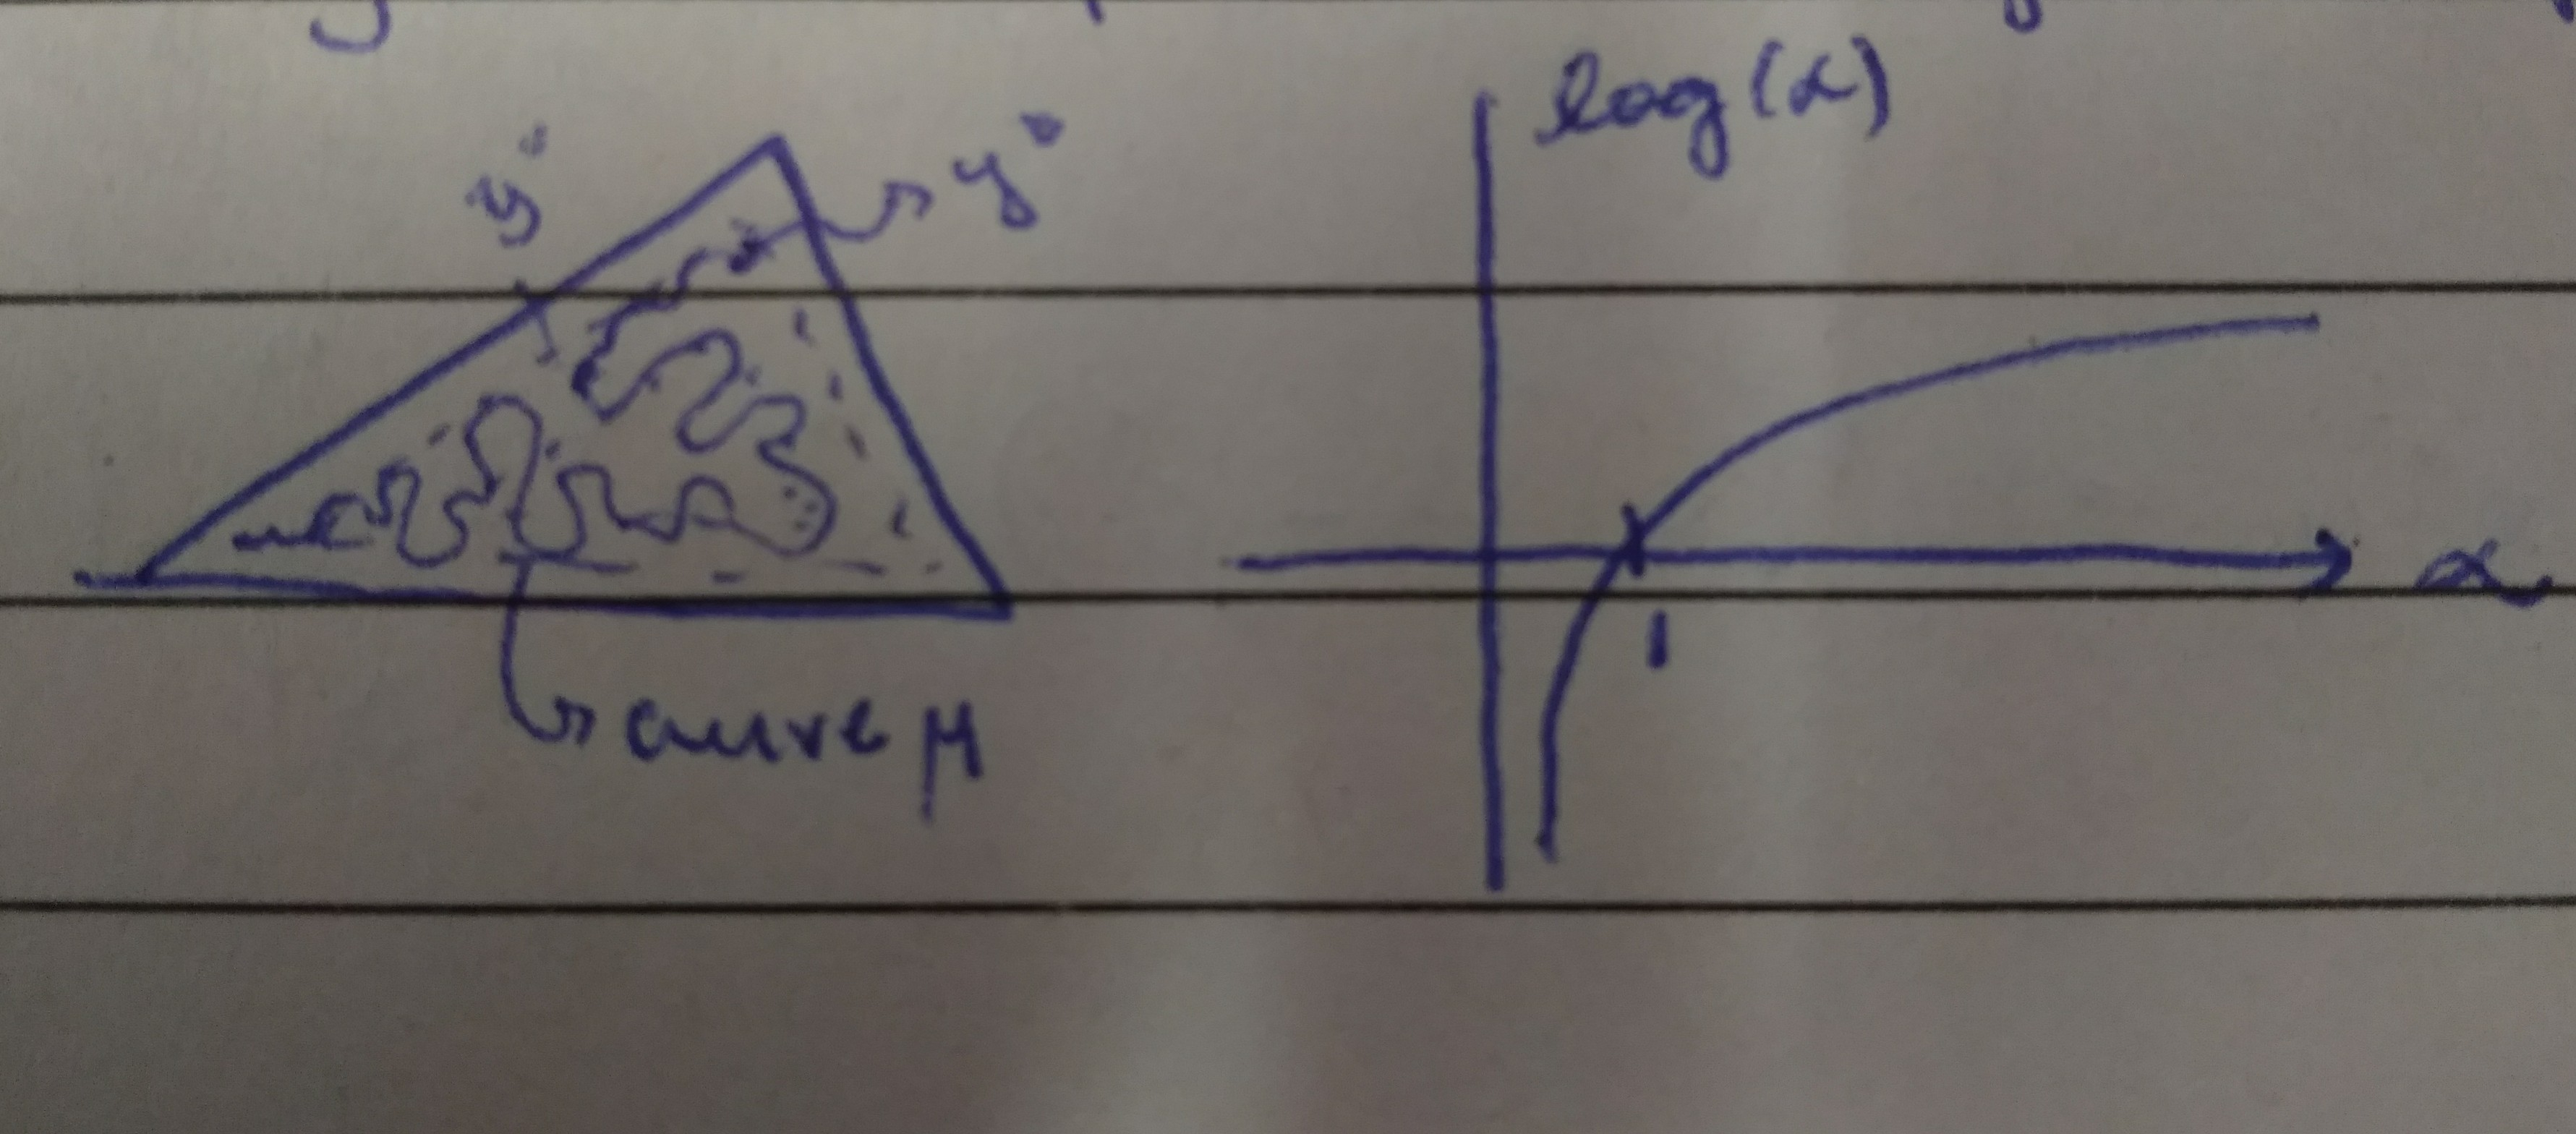
\includegraphics[width=0.3\textwidth]{imgs/interior-points.jpg}
\end{figure}

\begin{itemize}
\item For every $\mu > 0$, let $\Psi_\mu (y) = b^T y + \frac{1}{\mu}\phi(y)$
\item The curve $\mu \mapsto y^*(\mu) \in \mathbb{R}^m$. $y^*(\mu)$ is a point
that attains the minimum. $y^*(\mu) = \displaystyle \argmin_{y \in dom(\Psi_y)}
\Psi_mu(y)$ is called the central path.
\end{itemize}

\paragraph{Lemma:}
\begin{enumerate}
\item $dom(\Psi_\mu) = dom( \phi) = \{ y \in \mathbb{R}^m \mid y^T A > c \}$.
\item $\Psi_\mu$ is strictly convex (Hessian matrix).
\item $y^*(\mu)$ is uniquely defined.
\item $y^*(\mu)$ is striclty feasible for (D).
\item $\nabla \Psi_\mu (y^*(\mu)) = 0$.
\end{enumerate}

\subparagraph{Proof:}
\begin{enumerate}
\item obvious (related with log function)
\item $\nabla \phi(y) = - \sum_{j = 1}^{n} (\frac{1}{y^T A_{\cdot j} - c_j)}
A_{\cdot j}$.\\
$\nabla^2 \phi(y) = \sum_{j = 1}^{n} (\frac{1}{(y^T A_{\cdot j} - c_j)^2)}
(A_{\cdot j} A_{\cdot j}^T) \geq 0$, i.e, $\forall x \in \mathbb{R}^m\setminus
\{0\}$, $x^T \nabla^2 \phi(y) x \geq 0$: (PSD).\\
Assume $x^T \nabla^2 \phi(y)x = 0 \iff 0 = A_{\cdot j}^T x$ $\forall j \in
\{1, \dots, n\} \iff x \in ker(A^T)$, but this constradicts full row rank $A$,
unless $x = 0 \rightarrow \forall y \in dom(\phi)$: $\nabla^2 \phi(y) > 0
\rightarrow \phi$ is strictly convex $\rightarrow \Psi_\mu$ is strictly convex.
\item Claim: the minimum $\Psi_\mu(y)$ is attained in $\{y \in \mathbb{R}^m
\mid y^T A \geq \bar{c_j } \}$ (= $\bar{D}$), where $\bar{c_j}$ are some values
not the reduced cost.\\
(D) is bounded, $dom(\phi)$ is bounded, $\bar{D}$ is compact and convex. Then,
the statement 3 follows from preliminaries lemma.\\
Proof of the claim: $\underbrace{b^T y \text{is bounded over}
dom(\Psi_\mu)}_{\text{the domain itself is bounded}} \rightarrow \exists
\beta_j \in \mathbb{R}$ st $log(y^T A_{\cdot j} - c_j) \leq \beta_j$
$\forall y \in dom(\Psi_\mu)$ and $y_0 \in dom(\Psi_\mu)$ and
$k \in \{1, \dots, n\}$ we obtain $(*) b^T y - \sum_{j = \{1, \dots, n\}
\setminus k} \frac{1}{\mu} \beta_j - \frac{1}{\mu} log(\bar{c_k} - c_k)
\underbrace{>}_{\exists \bar{c_k}
\in \mathbb{R}} \Psi_\mu(y_0)$. This implies $\forall y \in dom(\Psi_\mu)$
$\Psi_\mu(y) \geq b^T y - \sum \frac{1}{\mu} \beta_j - \frac{1}{\mu} log(y^T
A_{\cdot k} - c_k) \geq (*) > \Psi_\mu(y_0)$.
\item clear
\item from lemma in preliminaries
\end{enumerate}

\paragraph{Lemma: let $\mu > 0$, the point $x^*(\mu)$ via $x^*(\mu) = \frac{1}
{\mu (y^*(\mu)^T A_{\cdot j} - c_j} \forall j$ satisfies:}

\begin{enumerate}
\item $x^*(\mu)$ is feasible for (P).
\item gap = $b^T y^*(\mu) - c^T x^*(\mu) = \frac{n}{\mu}$. We can choose $\mu$
so the gap between (P) and (D) is really small. The catch: must be possible to
find $y^*$.
\end{enumerate}

\subparagraph{Proof:}

\begin{enumerate}
\item $y^*(\mu)^T A_{\cdot j} - c_j > 0 \forall j \rightarrow x^*(\mu)j > 0$.\\
From previous lemma: $0 = \nabla \Psi_\mu(y^*(\mu)) = b - \sum_{j=1}^{n}
\frac{1 \times A_{\cdot j}}{\mu (y^*(\mu)^T A_{\cdot j} - c_j} = b -
\sum_{j=1}^{n} A_{\cdot j} x^*_j(\mu) = b - Ax^*(\mu) \rightarrow b =
Ax^*(\mu)$.
\item $y^*(\mu)^T b - x^*(\mu) = y^*(\mu)^T A x^*(\mu) - c^T x^* \mu =
(y^(\mu)^T A - c^T)x^*(\mu) = \sum_{j=1}^{n} (y^*(\mu)^T A_{\cdot j} -
c_j)x^*(\mu_j) \underbrace{=}_{\text{from $x^*(\mu)$ formula}} \sum_{j =1}^{n}
(\frac{1}{\mu} = \frac{n}{\mu}$.
\end{enumerate}

\paragraph{Our analysis allow us to formulate the Interior Point Algorithm:}
\begin{enumerate}
\item Choose $\mu_0 > 0$, $k >1$
\item Solve $y^*(\mu_0) = \displaystyle \argmin_{y \in dom(\Psi_{\mu_0})}
\Psi_{mu_0}(y)$.
\item For $t \geq 0$ do:
\subitem if $\frac{n}{\mu_t} \leq \epsilon$: quit
\subitem $\mu_{t+1} = k \mu_t$
\subitem solve $y^*(\mu_{t+1}) = \displaystyle \argmin_{y \in
dom(\Psi_{\mu_{t+1}})} \Psi_{mu_{t+1}}(y)$
\end{enumerate}

\paragraph{Lemma: Let $\epsilon > 0$. Suppose we can solve step 2 and 3 with
some oracle, then Integer Point Algorithm requires at most $T = \lceil
\frac{ln(\frac{n}{\mu_0 \epsilon})}{ln(k)} \rceil = \lceil log k
(\frac{n}{\mu_0 \epsilon}) \rceil$.}

\subparagraph{Proof:}
After $T$ iterations the gap is $\frac{n}{\mu_t} = \frac{n}{k^T \mu_0} =
\frac{n}{\lceil log k (\frac{n}{\mu_0 \epsilon}) \rceil \mu_0} \leq
\frac{n}{k^{log k(\frac{n}{\mu_o \epsilon})\mu_0}} =
\frac{n}{\frac{n}{\mu_0 \epsilon} \mu_0} = \epsilon$.
\end{document}